
\subsection{Llave electrónica transparente}

\label{section:switch}

El circuito cumple la función de una especie de compuerta OR analógica, poniendo a la salida tanto en el nivel de continua, como en el nivel de señal, el nivel de la terminal de entrada de mayor potencial.\\ 
El nivel de tensión continua a la salida, es prácticamente igual al nivel de tensión continua a la entrada, debido a las tensiones $V_{be}$ compensadas por las dos etapas, habrá una pequeña diferencia dada por las diferencias entre los transistores y diferencias en la corriente de colector.\\
La entrada con mayor potencial eleva el potencial en los emisores de los transistores internos de la llave, $Q_{7}$ y $Q_{8}$, y hace que se corte el transistor de la entrada con menor potencial. \\
Otra cosa importante es que la llave es perfectamente simétrica, si las tensiones de entrada se invierten, los puntos de trabajo de los transistores de cada mitad de la llave se invierten.\\
A los efectos de señal para la terminal de entrada que comande la salida, son dos seguidores en cascada, esto sumado a lo dicho en el párrafo anterior, justifica hablar de una llave trasparente. Otro detalle importante, es que por tratarse de dos seguidores en cascada, se tiene una impedancia muy alta de entrada, cargando muy poco a los circuitos conectados a las entradas.\\
Utilizamos el circuito mostrado en la figura~\figref{fig:fig_analogic_switch}, para simular su comportamiento, utilizando en una de sus entradas un valor de continua fijo, $1 \si[per-mode=symbol]{\volt}$, y una señal cuadrada de $1.1 \si[per-mode=symbol]{\volt}$ de pico y $500 \si[per-mode=symbol]{\hertz}$ en su otra entrada. Se eligió una frecuencia de un valor tal que se puedan observar algunos efectos reactivos en el circuito. Se realizó una simulación de tipo transitorio con el comando \textbf{SPICE} \textit{.tran}, el resultado se exportó y se graficó en \textbf{MATLAB}, el resultado de la simulación se puede ver en la figura~\figref{fig:fig_analogic_switch_simulation}, se puede observar claramente como la salida sigue a la entrada de la llave con mayor potencial, y se pueden observar también los efectos reactivos, mayormente debidos a la discontinuidad de la señal en una de las entradas.\\
En cuanto al ancho de banda del circuito, por tratarse de una cascada de dos seguidores, tendremos que el ancho de banda será seguramente limitado por las bases de los transistores, en particular el transistor exterior que este activo, al tener una gran resistencia de entrada, y si el el circuito de entrada agrega capacidad a este nodo, sin duda será este el nodo limitante, pero si no es el caso y solo influyen las capacidades parásitas de los transistores, se puede esperar un ancho de banda de varios $\si[per-mode=symbol]{\mega\hertz}$, en particular para este circuito sin cargas o entradas capacitivas, realizando una simulación con el comando \texttt{SPICE} \textit{.ac} desde la entrada activa, se obtuvo $36.1 \si[per-mode=symbol]{\mega\hertz}$.


\vfill

\clearpage

\begin{figure}[H] %htb
\begin{center}
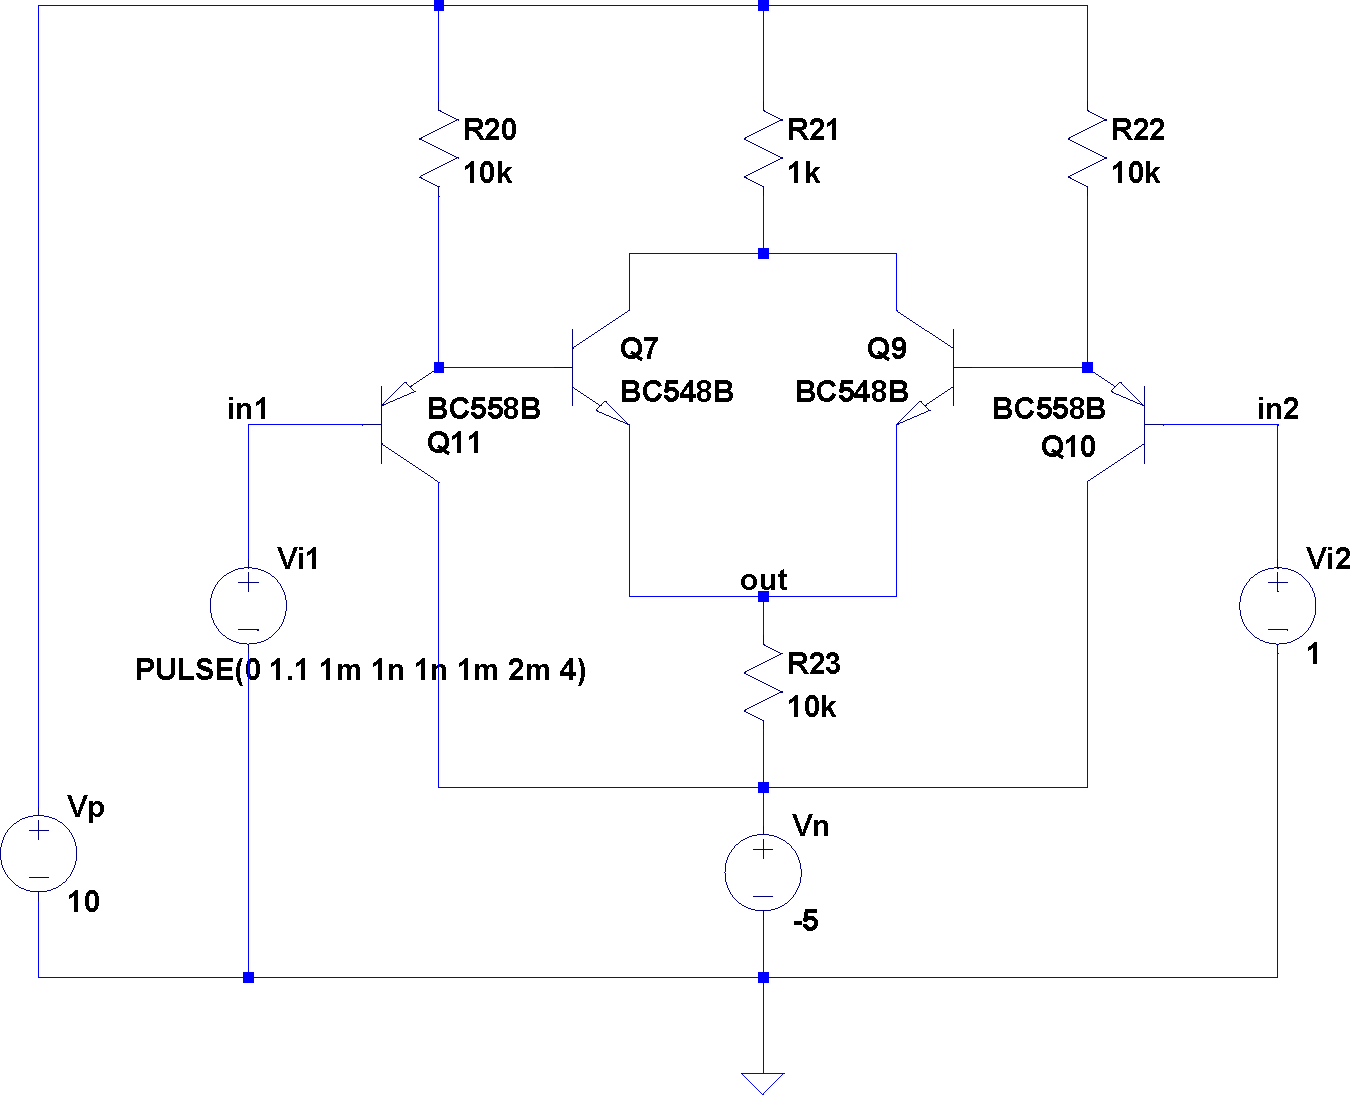
\includegraphics[width=1 \textwidth, angle=0]{./img/llave/OR-Q7-9-10-11.png}
\caption{\label{fig:fig_analogic_switch}\footnotesize{Circuito utilizado para simular la llave analógica.}}
\end{center}
\end{figure}

\vfill

\clearpage


\begin{figure}[H] %htb
\begin{center}
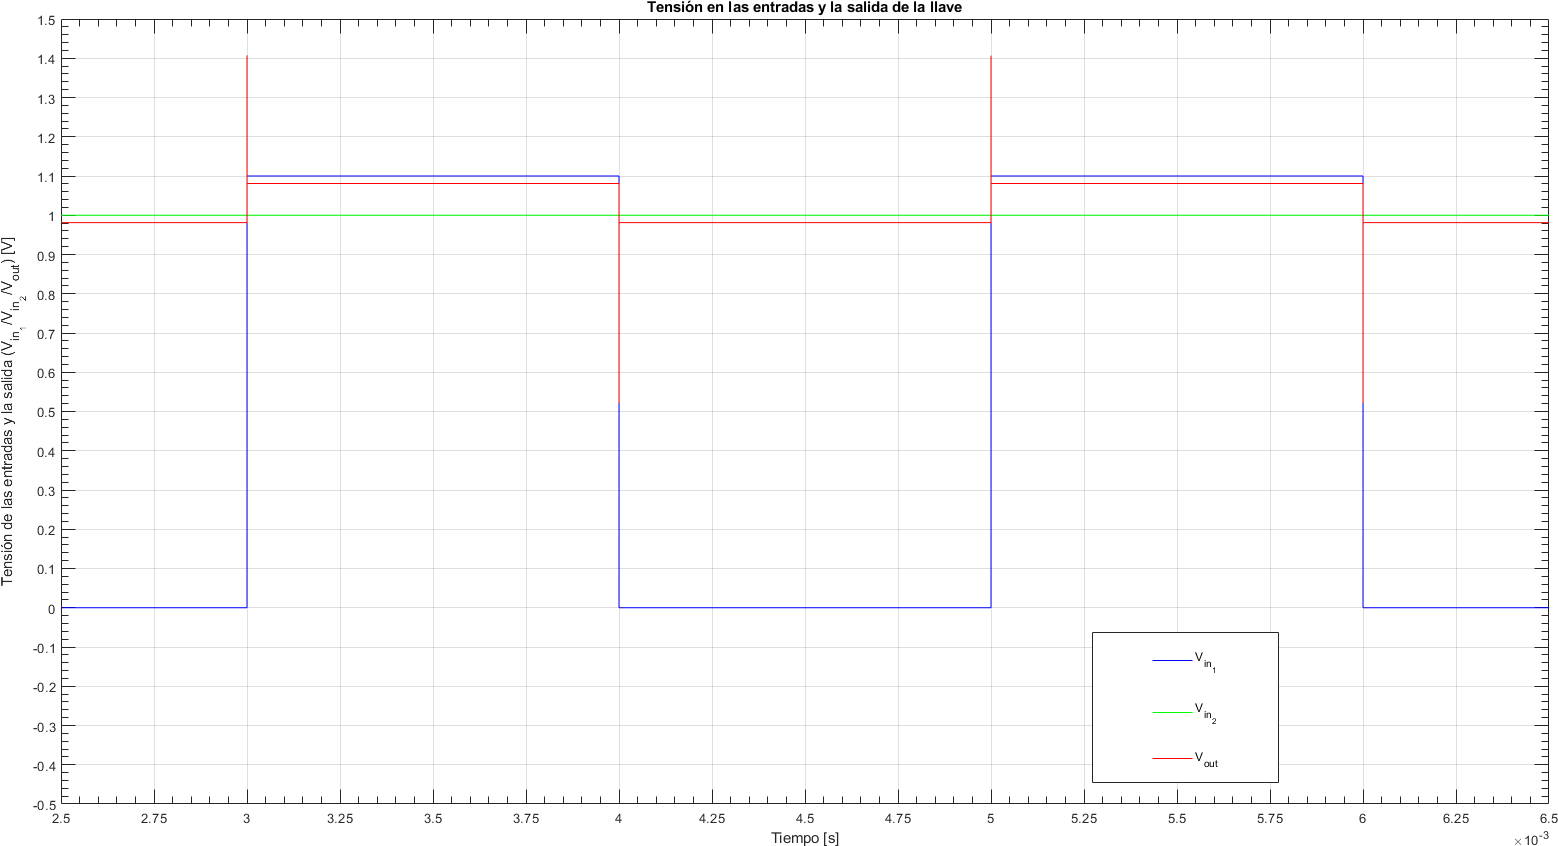
\includegraphics[width=1.2 \textwidth, angle=90]{./img/llave/switch_response.png}
\caption{\label{fig:fig_analogic_switch_simulation}\footnotesize{Respuesta de la llave analógica.}}
\end{center}
\end{figure}

\clearpage